%ATC_example
\begin{figure}[t]
\centering
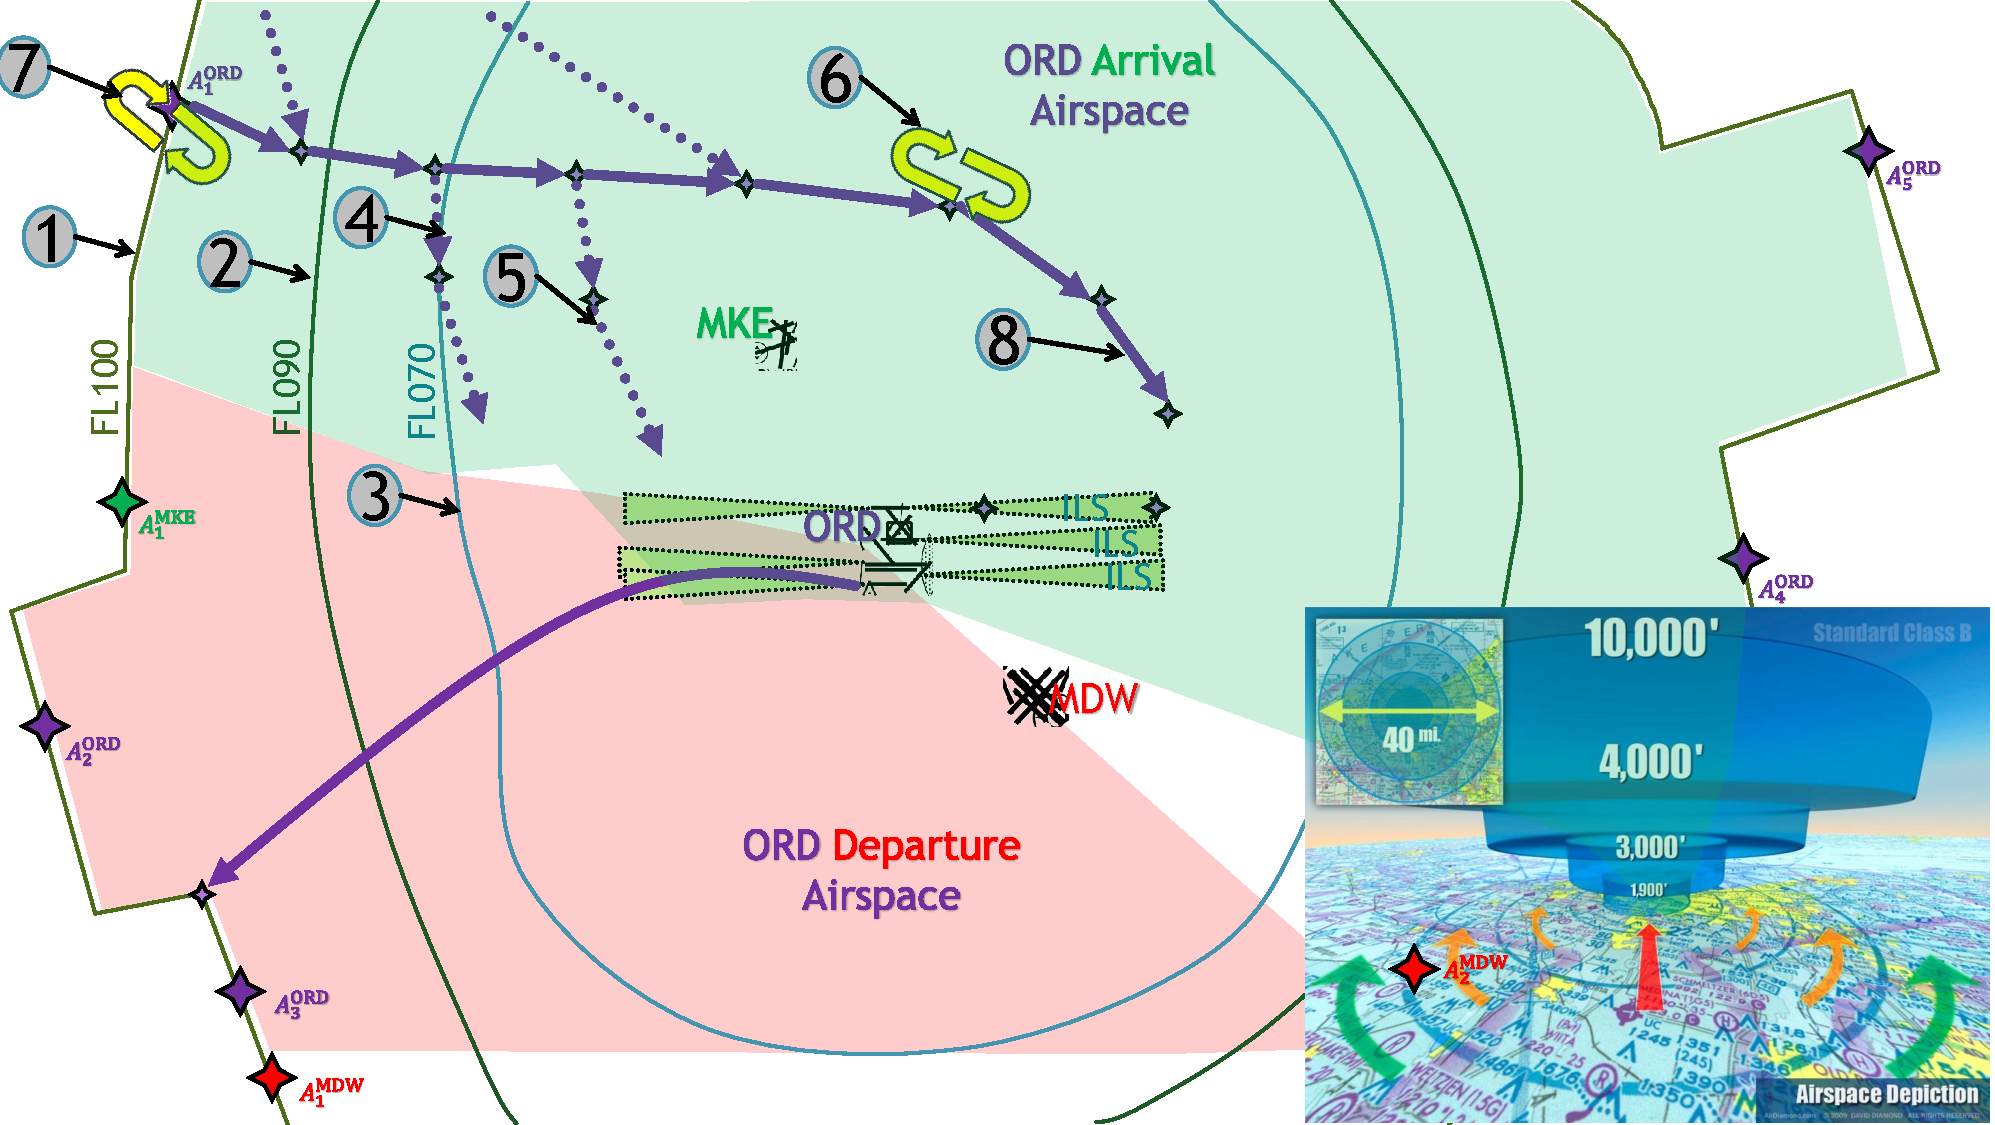
\includegraphics[width=0.49\textwidth]{figures/ATC_Example}
%\vspace{-10pt}
\caption{{\small A simplified depiction of Chicago O'Hare (ORD) airport and its airspace.  Figure courtesy Max Z. Li, Univ. of Pennsylvania.}}
\label{fig:atc_example}
%\vspace{-20pt}
\end{figure}


\textbf{Motivating example.} A particular system with complex rules and applicable to multiple dynamic objects is Air-Traffic Control (ATC) for landing arrivals at an airport. Fig. \ref{fig:atc_example} depicts the Chicago O'Hare (ORD) area airspace, with a radius of $40$ miles. In the arrival airspace are 3 zones with different, hierarchical, altitude floors and ceilings. It also shows holding zones, landing approaches, and allowable trajectories/ for the landing. The following is a subset of the simplified rules that apply for incoming air-crafts, some numbered in red-circles in Fig. \ref{fig:atc_example}:

\begin{itemize}
\vspace{-5pt}
\item An incoming aircraft has to follow a prescribed sequence of way-points.
\vspace{-5pt}
\item $1$, $2$ and $3$ mark three Zones, FL100, FL90 and FL70 with altitude ceilings of $10000$, $9000$ and $7000$ feet, and floors of $4000$, $3000$ and $1900$ feet respectively.
\vspace{-5pt}
\item $4$ and $5$ show two trajectories which have been assigned either one of two runways that allow landings from that direction. $8$ shows a trajectory for an air-craft assigned to land in the other direction, e.g. in case of adverse weather.
\vspace{-5pt}
\item $6$ and $7$ show two holding zones, one at the outer Zone (FL100) and the other in the inner-most zone (FL70). An air-craft could be assigned to a holding zone in case the air-space is too busy.
\vspace{-5pt}
\item ATC is responsible for maintaining a minimum separation between air-crafts in the airspace.
\vspace{-5pt}
\end{itemize}

Thee are just a subset of the actual set of rules for ATC in the arrival area. Since all air-crafts entering the airspace have to be landed in a timely manner, these ATC arrival airspace rules can be formalized as a timed MTL formula. In a case study later in the paper (\ref{sec:ATCquad}), we formalize a version of such rules for of ATC for autonomous quad-rotors.

